\documentclass[a4paper,12pt]{article}
\usepackage{amsmath}
\usepackage{amssymb}
\usepackage[polish]{babel}
\usepackage{polski}
\usepackage[utf8]{inputenc}
\usepackage{indentfirst}
\usepackage{geometry}
\usepackage{array}
\usepackage[pdftex]{color,graphicx}
\usepackage{subfigure}
\usepackage{afterpage}
\usepackage{setspace}
\usepackage{color}
\usepackage{wrapfig}
\usepackage{listings}
\usepackage{datetime}

\renewcommand{\onehalfspacing}{\setstretch{1.6}}

\geometry{tmargin=2.5cm,bmargin=2.5cm,lmargin=2.5cm,rmargin=2.5cm}
\setlength{\parindent}{1cm}
\setlength{\parskip}{0mm}

\newenvironment{lista}{
\begin{itemize}
  \setlength{\itemsep}{1pt}
  \setlength{\parskip}{0pt}
  \setlength{\parsep}{0pt}
}{\end{itemize}}

\newcommand{\linia}{\rule{\linewidth}{0.4mm}}

\definecolor{lbcolor}{rgb}{0.95,0.95,0.95}
\lstset{
    backgroundcolor=\color{lbcolor},
    tabsize=4,
  language=C++,
  captionpos=b,
  tabsize=3,
  frame=lines,
  numbers=left,
  numberstyle=\tiny,
  numbersep=5pt,
  breaklines=true,
  showstringspaces=false,
  basicstyle=\footnotesize,
  identifierstyle=\color{magenta},
  keywordstyle=\color[rgb]{0,0,1},
  commentstyle=\color{Darkgreen},
  stringstyle=\color{red}
  }

\begin{document}

\noindent
\begin{tabular}{|c|p{11cm}|c|} \hline 
Grupa 6 & Dariusz Szczupak, Kamil Wanat & \ddmmyyyydate\today \tabularnewline
\hline 
\end{tabular}


\section*{Zadanie 2 - Rozmycie Gaussa w MPI}

Celem zadania jest program oparty na algorytmie Gaussa mający na celu rozmycie danego zdjęcia. Zadanie wykonane z wykorzstaniem standardu MPI. "Gauss 2" - to użyta wersja filtru danego w dołączonym do treści zadania linku. Maska w danym filtrze wygląda następująco:

\begin{lstlisting}
int mask[5][5] = {{1,1,2,1,1}, {1,2,4,2,1}, {2,4,8,4,2}, {1,2,4,2,1}, {1,1,2,1,1}
};
\end{lstlisting}

Do obliczenia wartości z których składa się każdy piksel(Red, Green, Blue), potrzebne są punkty otaczające go. Każdy taki piksel ma jakąś wage, która z kolei zapisana jest w masce filtra. Liczymy sume ważoną kolejnych pixeli i jego sąsiadów, kolejnie dzielimy taką sumę przez sumę całej maski. Filtrowanie obrazu następuje oddzielnie dla każdej wartości z której składa się pixel. W metodzie filtrowania Gaussa znaczenie wartości pixela jest największe w punkcie, który jest liczony i zmniejsza się wraz z oddalaniem się od niego. Poniżej przesyłanie czesci danych pomiedzy procesami:

\begin{lstlisting}
comm = MPI_COMM_WORLD;
    MPI_Comm_rank(comm, &rank);
    MPI_Comm_size(comm, &size); 
    if (rank == 0) { 
for (int i = 1; i < size; i++) {
            if (i == (size - 1))
                width = img.cols - start;
            slice = Mat(width, img.rows, CV_8UC3);
            slice = img(Rect(start, 0, width, img.rows)).clone();
            start = end - 4;
            end = start + width;

            int sliceColumn = slice.cols;
            int sliceRows = slice.rows;
            
            MPI_Send(&sliceColumn, 1, MPI_INT, i, 0, comm);
            MPI_Send(&sliceRows, 1, MPI_INT, i, 1, comm);
            MPI_Send(slice.data, sliceColumn * sliceRows * 3, MPI_BYTE, i, 2, comm);
        }

for (int i = 1; i < size; i++) {
            int tempcols, temprows;
            MPI_Recv(&tempcols, 1, MPI_INT, i, 0, comm, MPI_STATUS_IGNORE);
            MPI_Recv(&temprows, 1, MPI_INT, i, 1, comm, MPI_STATUS_IGNORE);
            Mat tempimg = Mat(temprows, tempcols, CV_8UC3);
            MPI_Recv(tempimg.data, tempcols * temprows * 3, MPI_BYTE, i, 2, comm, MPI_STATUS_IGNORE);
            if (i == 1) {
                imgScore = tempimg.clone();
            } else {
                hconcat(imgScore, tempimg, imgScore);
            }
          }  
        }        
\end{lstlisting}

Na wstępie proces macierzysty (rank == 0) dzieli obrazek na paski, a następnie rozsyła je równomiernie do wszystkich pozostałych procesów. Po przetworzeniu dane w postaci pasów pikseli zostają poskładane w nowy obraz. Rozwiązanie to pozwala na maksymalne wykorzystanie dostepnych procesów.

\begin{figure}[!hbp]
	\centering
  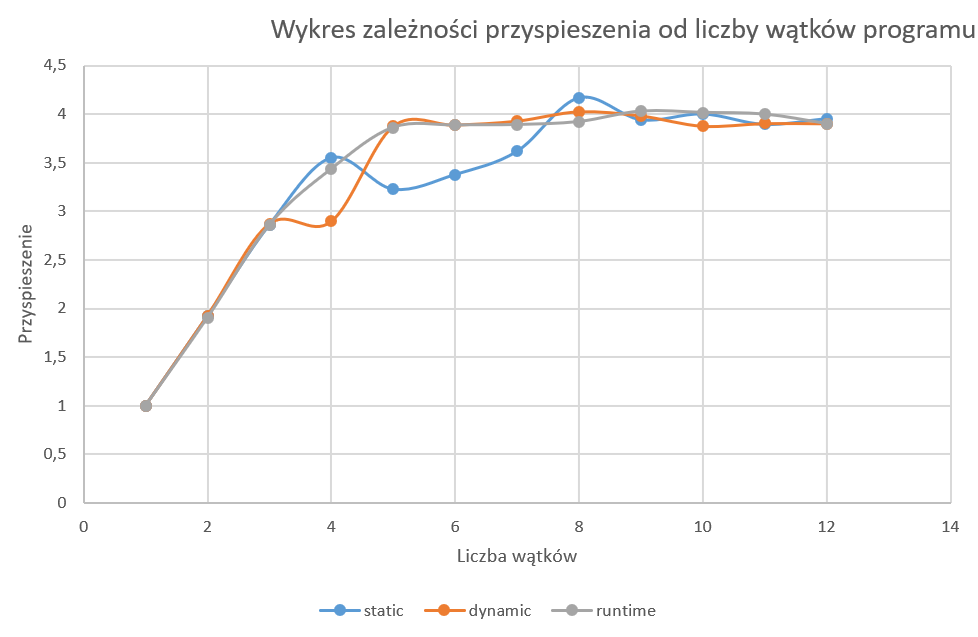
\includegraphics[width=0.7\textwidth]{wykres1.png}
  \caption{Wykres przyspieszenia}
\end{figure}


\begin{wrapfigure}{r}{0.5\textwidth}
  \vspace{-20pt}
  \begin{center}
  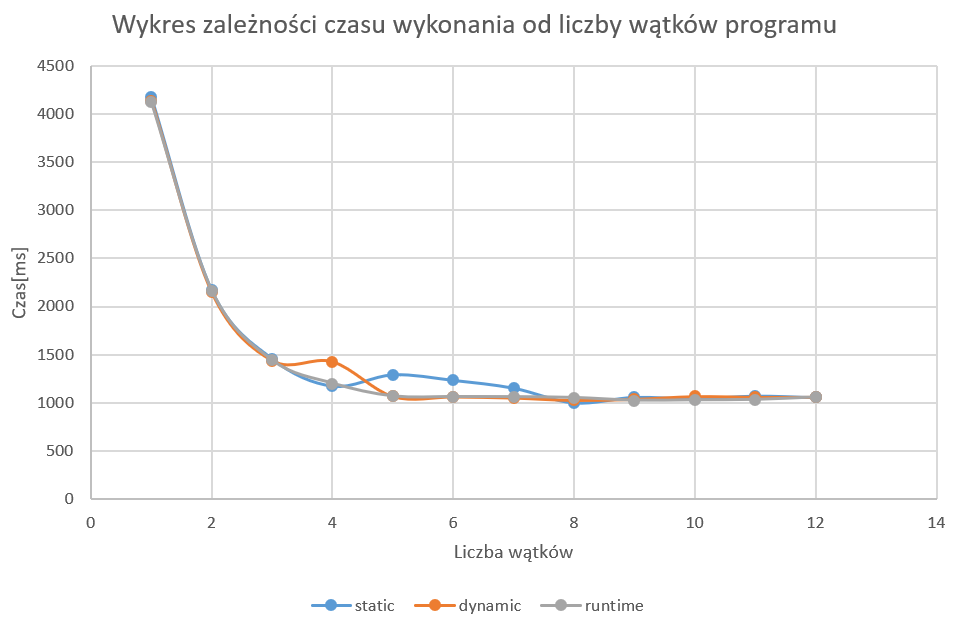
\includegraphics[width=0.45\textwidth]{wykres.png}
  \end{center}
  \vspace{-20pt}
  \caption{Wykres zależności czasu od liczby wątków}
  \vspace{-10pt}
\end{wrapfigure}

Z powyższych wykresów można wywnioskować że czas obliczeń spada gwałtownie miedzy 2 a 3 procesem po czym następuje stabilizacja.

Dane przeprowadzanych testów:
\begin{lista}
 \item Wzięto pod uwagę średnią pomiarów czasów wykonania programu dla liczby wątków z przedziału od 2 do 13. Program był uruchamiany dla obrazka ściągniętego z przestworzy internetów w rozdzielczośći 1920x1200px.
 \item Do mierzenia czasu wykorzystano MPIWtime.
 \item Do wczytania obrazu wykorzystano bibliotekę OpenCV .
 \item Testy zostały wykonane na serwerze cuda.iti.pk.edu.pl . 
\end{lista}
 
Zapoznaliśmy się z protokołem MPI. Zadanie udało się wykonać w całości. Wniosek nasuwa się taki, iż za pomocą MPI można przyspieszyć czas obliczeń algorytmu rozmycia Gaussa. Najlepsze wyniki osiągnięto dla ilości wątków zbliżonej do ilości rdzeni procesora na serwerze CUDA. 


\end{document}